\documentclass[12pt,letterpaper]{article}
\usepackage{graphicx,textcomp}
\usepackage{natbib}
\usepackage{setspace}
\usepackage{fullpage}
\usepackage{color}
\usepackage[reqno]{amsmath}
\usepackage{amsthm}
\usepackage{fancyvrb}
\usepackage{amssymb,enumerate}
\usepackage[all]{xy}
\usepackage{endnotes}
\usepackage{lscape}
\newtheorem{com}{Comment}
\usepackage{float}
\usepackage{hyperref}
\newtheorem{lem} {Lemma}
\newtheorem{prop}{Proposition}
\newtheorem{thm}{Theorem}
\newtheorem{defn}{Definition}
\newtheorem{cor}{Corollary}
\newtheorem{obs}{Observation}
\usepackage[compact]{titlesec}
\usepackage{dcolumn}
\usepackage{tikz}
\usetikzlibrary{arrows}
\usepackage{multirow}
\usepackage{xcolor}
\newcolumntype{.}{D{.}{.}{-1}}
\newcolumntype{d}[1]{D{.}{.}{#1}}
\definecolor{light-gray}{gray}{0.65}
\usepackage{url}
\usepackage{listings}
\usepackage{color}

\definecolor{codegreen}{rgb}{0,0.6,0}
\definecolor{codegray}{rgb}{0.5,0.5,0.5}
\definecolor{codepurple}{rgb}{0.58,0,0.82}
\definecolor{backcolour}{rgb}{0.95,0.95,0.92}

\lstdefinestyle{mystyle}{
	backgroundcolor=\color{backcolour},   
	commentstyle=\color{codegreen},
	keywordstyle=\color{magenta},
	numberstyle=\tiny\color{codegray},
	stringstyle=\color{codepurple},
	basicstyle=\footnotesize,
	breakatwhitespace=false,         
	breaklines=true,                 
	captionpos=b,                    
	keepspaces=true,                 
	numbers=left,                    
	numbersep=5pt,                  
	showspaces=false,                
	showstringspaces=false,
	showtabs=false,                  
	tabsize=2
}
\lstset{style=mystyle}
\newcommand{\Sref}[1]{Section~\ref{#1}}
\newtheorem{hyp}{Hypothesis}

\title{Problem Set 1}
\date{Due: September 30, 2024}
\author{Applied Stats/Quant Methods 1}

\begin{document}
	\maketitle
	
	\section*{Instructions}
	\begin{itemize}
	\item Please show your work! You may lose points by simply writing in the answer. If the problem requires you to execute commands in \texttt{R}, please include the code you used to get your answers. Please also include the \texttt{.R} file that contains your code. If you are not sure if work needs to be shown for a particular problem, please ask.
\item Your homework should be submitted electronically on GitHub.
\item This problem set is due before 23:59 on Monday September 30, 2024. No late assignments will be accepted.
%\item Total available points for this homework is 80.
	\end{itemize}
	
	\vspace{1cm}
	\section*{Question 1: Education}

A school counselor was curious about the average of IQ of the students in her school and took a random sample of 25 students' IQ scores. The following is the data set:\\
\vspace{.5cm}

\lstinputlisting[language=R, firstline=5, lastline=5]{PS01_answersSL.R}  

\vspace{1cm}
\begin{enumerate}
	\item Find a 90\% confidence interval for the average student IQ in the school.\\
	
	First I calculated n using 
	\begin{verbatim}
		> length(dataset_edu)
	\end{verbatim}
	
	Since n is smaller than 30 and I do not know the standard deviation of the whole sample, I decided to calculate the confidence interval using a t-distribution. To do so, I first calculated the t-score:
\begin{verbatim}
	> t_score <- qt(0.95, df=25-1)
		\end{verbatim}

	then I calculated the confidence interval
	\begin{verbatim}
	> conf_high <- mean(dataset_edu)+(t_score)*(sd(dataset_edu)/sqrt(25))
	> conf_low <- mean(dataset_edu)-(t_score)*(sd(dataset_edu)/sqrt(25))
	> conf_high
	[1] 102.9201
	> conf_low
	[1] 93.95993
		\end{verbatim}
	Thus, the 90\% confidence interval is: [93.96; 102.92]
	
	\item Next, the school counselor was curious  whether  the average student IQ in her school is higher than the average IQ score (100) among all the schools in the country.\\ 
	
	\noindent Using the same sample, conduct the appropriate hypothesis test with $\alpha=0.05$.\\ 
	
	H1: higher than average (meaning the H1 is one-sided)
	
	H0: lower than or equal to average 
		\begin{verbatim}
	> t.test(dataset_edu, mu = 100, alternative = "greater")
	
	One Sample t-test
	
	data:  dataset_edu
	t = -0.59574, df = 24, p-value = 0.7215
	alternative hypothesis: true mean is greater than 100
	95 percent confidence interval:
	93.95993      Inf
	sample estimates:
	mean of x 
	98.44 
		\end{verbatim}
	
	The p-value = 0.7215
	
	0.7215 is a higher value than 0.05, therefore we reject our alternative hypothesis (alternative hypothesis= the average student IQ in her school is higher than the average IQ score among all the schools in the country.)
\end{enumerate}

\newpage

	\section*{Question 2: Political Economy}

\noindent Researchers are curious about what affects the amount of money communities spend on addressing homelessness. The following variables constitute our data set about social welfare expenditures in the USA. \\
\vspace{.5cm}


\begin{tabular}{r|l}
	\texttt{State} &\emph{50 states in US} \\
	\texttt{Y} & \emph{per capita expenditure on shelters/housing assistance in state}\\
	\texttt{X1} &\emph{per capita personal income in state} \\
	\texttt{X2} &  \emph{Number of residents per 100,000 that are "financially insecure" in state}\\
	\texttt{X3} &  \emph{Number of people per thousand residing in urban areas in state} \\
	\texttt{Region} &  \emph{1=Northeast, 2= North Central, 3= South, 4=West} \\
\end{tabular}

\vspace{.5cm}
\noindent Explore the \texttt{expenditure} data set and import data into \texttt{R}.
\vspace{.5cm}

\vspace{.5cm}
\begin{itemize}

\item
Please plot the relationships among \emph{Y}, \emph{X1}, \emph{X2}, and \emph{X3}? What are the correlations among them (you just need to describe the graph and the relationships among them)?


First I created a 3x2 grid layout using 
	\begin{verbatim}
		> par(mfrow = c(3, 2))
			\end{verbatim}
then I plotted all individual plots into that grid:
\begin{verbatim}
	> plot(expenditure$X1, expenditure$Y,  main = "Relationship between X1 and Y",  
	+      xlab = "per capita personal income in state", 
	+      ylab = "/capita expenditure shelters/housing assistance")
	> plot(expenditure$X2, expenditure$Y,  main = "Relationship between X2 and Y",  
	+      xlab = "number residents/100,000 ”financially insecure” in state", 
	+      ylab = "/capita expenditure shelters/housing assistance")
	> plot(expenditure$X3, expenditure$Y,  main = "Relationship between X3 and Y",  
	+      xlab = "number people/1000 residing in urban areas in state", 
	+      ylab = "/capita expenditure shelters/housing assistance")
	> plot(expenditure$X1, expenditure$X2, main = "Relationship between X1 and X2", 
	+      xlab = "per capita personal income in state", 
	+      ylab = "number residents/100,000 ”financially insecure”")
	> plot(expenditure$X1, expenditure$X3, main = "Relationship between X1 and X3", 
	+      xlab = "per capita personal income in state", 
	+      ylab = "number people/1000 residing in urban areas")
	> plot(expenditure$X2, expenditure$X3, main = "Relationship between X2 and X3", 
	+      xlab = "number residents/100,000 ”financially insecure”", 
	+      ylab = "number people/1000 residing in urban areas")
		\end{verbatim}
		
I had to shorten some of the names of the scales to fit in the graph. Please assume every scale to refer to the situation "in state".


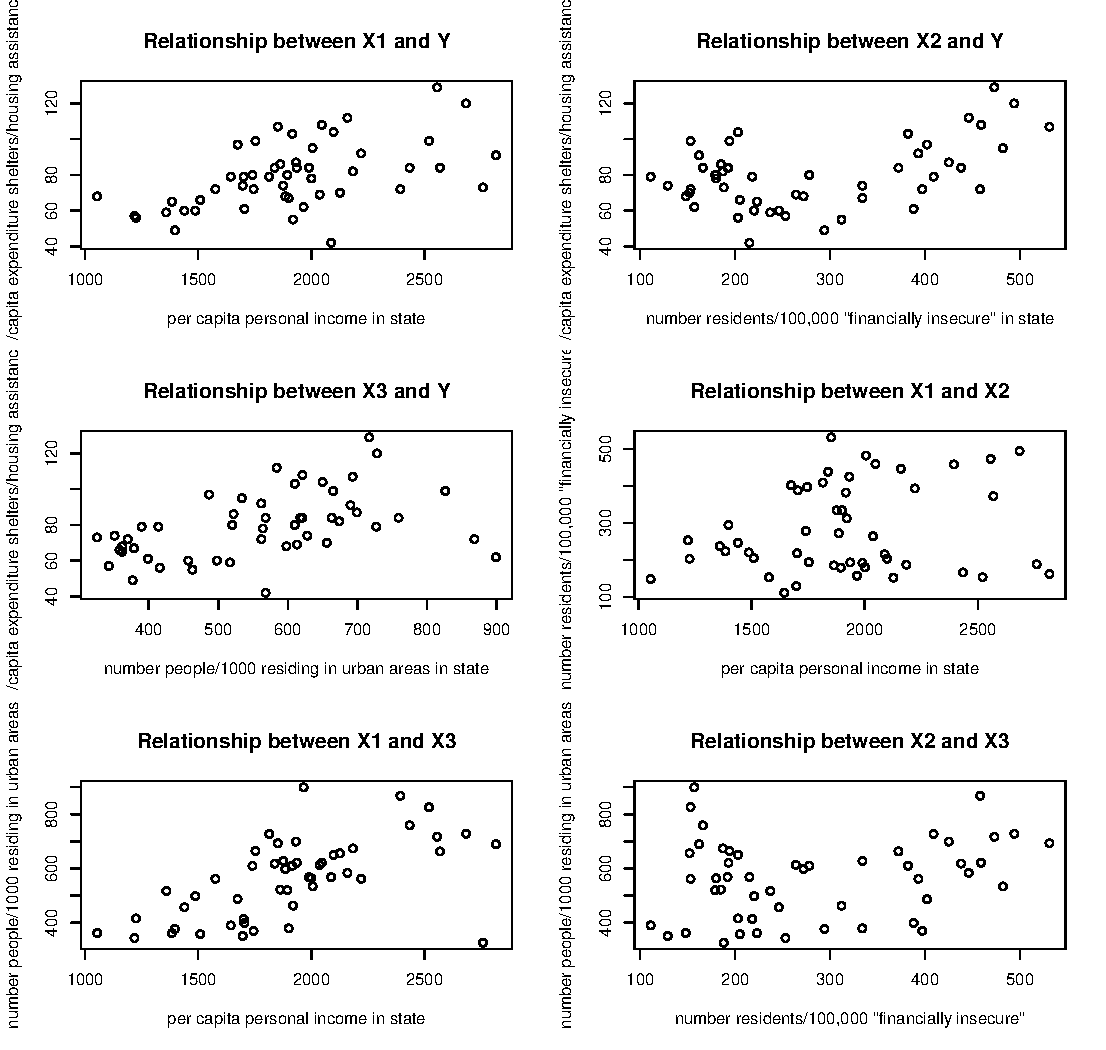
\includegraphics[width=\textwidth,height=\textheight,keepaspectratio]{Plot_X_Y}

I don't find any of the correlations to be very clear-cut linear correlations. However, the first graph (Relationship between X1 and Y) shows what I would consider still a linear correlation throughout the whole graph, especially a the most frequent values for X1 (X1=1500-2000). The relationship between X2 and Y seems to be linear starting at about X2=200. Before that the distribution seems almost U-shaped. The relationship between X3 and Y appear linear to me as well, however the highest X3-values (X3=800-900) seem to have lower Y-values again. Since there are not many observation like this, I would still consider the overall distribution linear. The distribution between X1 and X3 also appears to be linear, while the relationship between X1 and X2 as well as between X2 and X3 seems to have, in my opinion, no discernible distribution, linear or otherwise. In general, I believe more observations would be helpful in determining linearity, especially in the case of X3 and Y. 

\vspace{.5cm}
\item
Please plot the relationship between \emph{Y} and \emph{Region}? On average, which region has the highest per capita expenditure on housing assistance?

To do so I created a boxplot, since it is easiest to see relevant values like median or maximum value in that kind of graph.
\begin{verbatim}
	boxplot(Y ~ Region, data = expenditure,
	xlab="Region",
	ylab="per capita expenditure on shelters/housing assistance in state",
	main="Relationship between Region and Y")
		\end{verbatim}

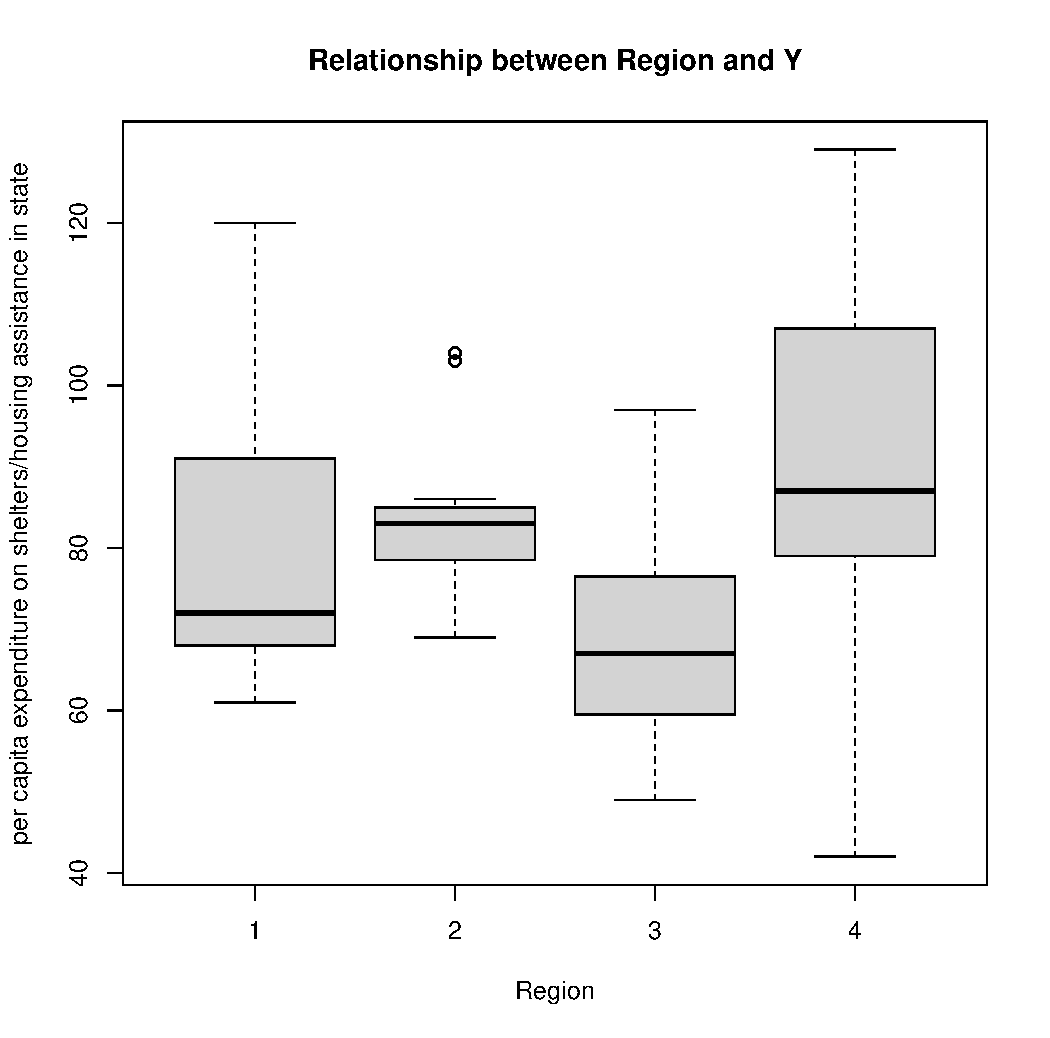
\includegraphics{Boxplot_Region_Y}
Region 4 (West) seems to have the highest median (shown by the black line), followed by Region 2 (North Central). However the maximum values of Y can be found in Region 4 and Region 1 (Northeast), not Region 2. So overall, I think the highest per capita expenditure on housing assistance can be found in the West. 
\vspace{.5cm}
\item
Please plot the relationship between \emph{Y} and \emph{X1}? Describe this graph and the relationship. Reproduce the above graph including one more variable \emph{Region} and display different regions with different types of symbols and colors.

First, plotting the relationship between Y and X1:
\begin{verbatim}
> plot(expenditure$X1,expenditure$Y, 
+      xlab = "per capita personal income in state",
+      ylab = "per capita expenditure on shelters/housing assistance in state", 
+      main = "Relationship between X1 and Y") 
\end{verbatim}
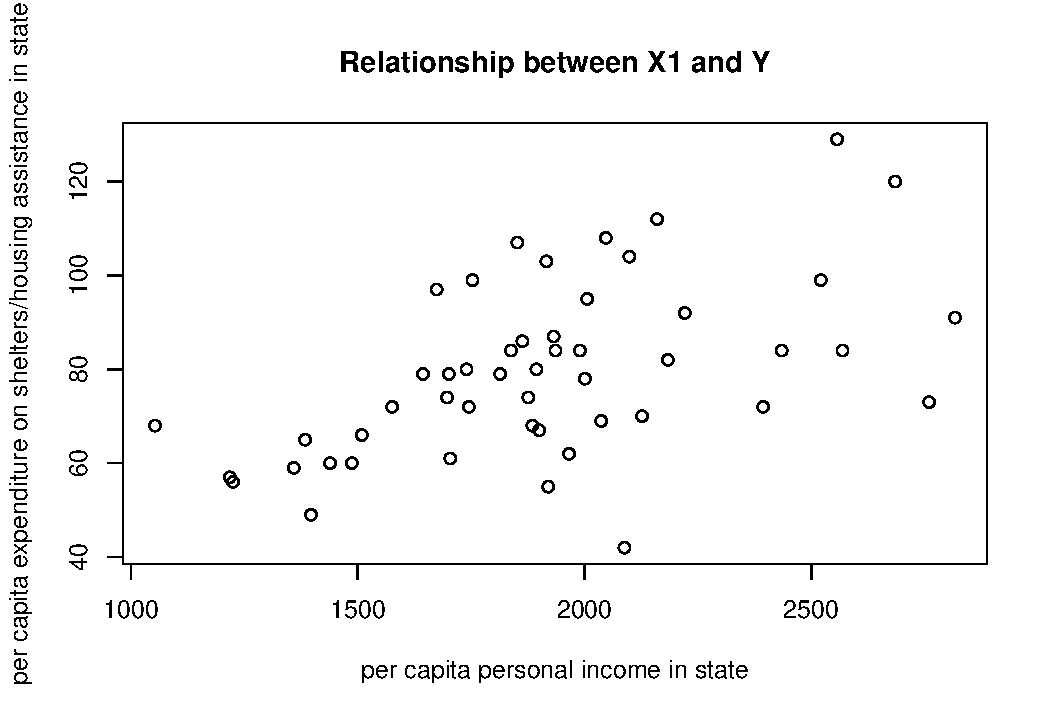
\includegraphics[width=\textwidth,height=\textheight,keepaspectratio]{Plot_X1_y}
As I answered before, the relationship between X1 and Y according to this scatterplot seems positively linear to me. The higher the per capita personal income in a state, the higher the per capita expenditure on shelters/housing assistance in that state. This can be seen especially where there are a lot of observations (around X1=1500-2000). However, there are not a lot of observations so it is difficult to tell, especially when considering the states with a higher per capita personal income (X1=2500 or more).


After that, I add the variable "Region"

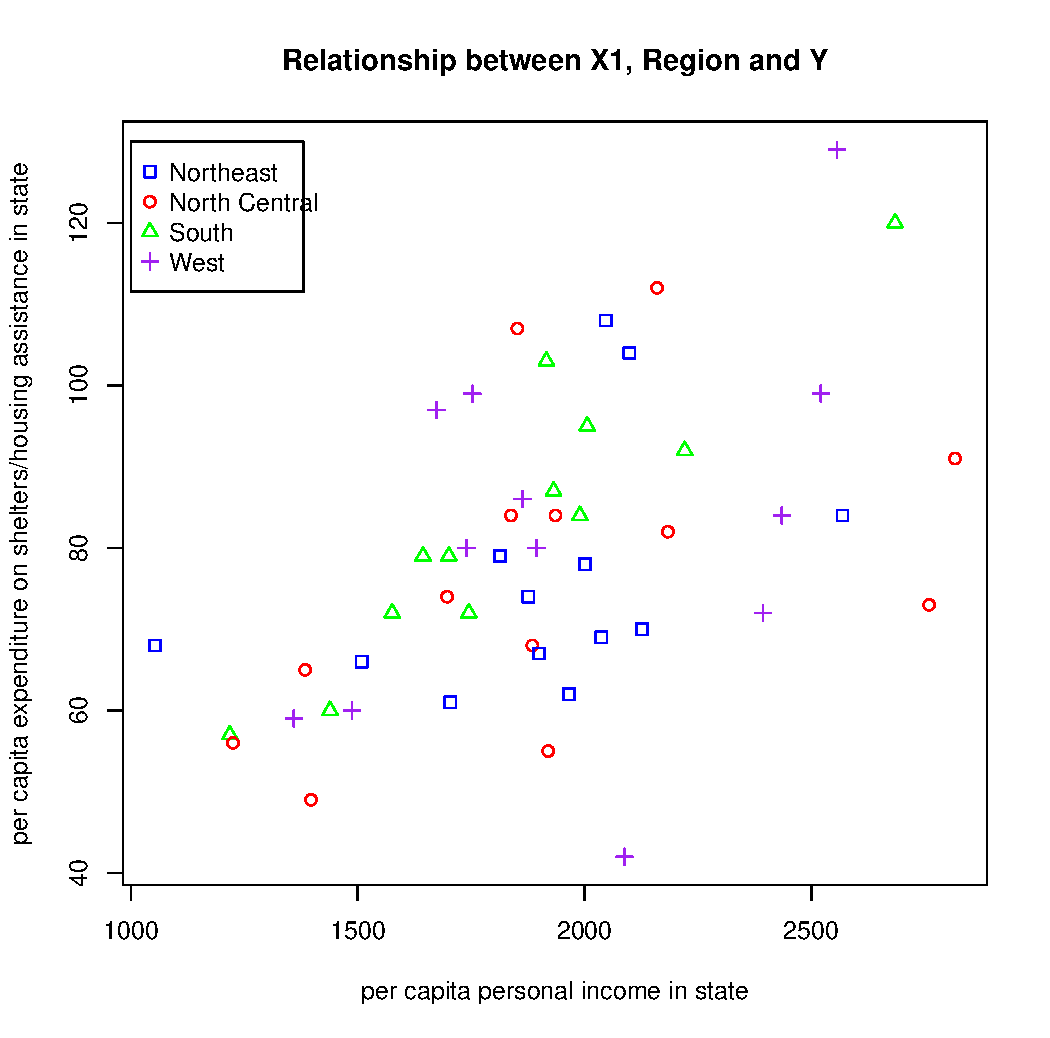
\includegraphics[width=\textwidth,height=\textheight,keepaspectratio]{Plot_X1_Region_Y}
\end{itemize}


\end{document}
